\documentclass[a4paper]{article}

\def\npart {II}
\def\nterm {Lent}
\def\nyear {2017}
\def\nlecturer {H. S. Reall}
\def\ncourse {Statistical Physics}

% Imports
\ifx \nextra \undefined
  \usepackage[pdftex,
    hidelinks,
    pdfauthor={Dexter Chua},
    pdfsubject={Cambridge Maths Notes: Part \npart\ - \ncourse},
    pdftitle={Part \npart\ - \ncourse},
  pdfkeywords={Cambridge Mathematics Maths Math \npart\ \nterm\ \nyear\ \ncourse}]{hyperref}
  \title{Part \npart\ - \ncourse}
\else
  \usepackage[pdftex,
    hidelinks,
    pdfauthor={Dexter Chua},
    pdfsubject={Cambridge Maths Notes: Part \npart\ - \ncourse\ (\nextra)},
    pdftitle={Part \npart\ - \ncourse\ (\nextra)},
  pdfkeywords={Cambridge Mathematics Maths Math \npart\ \nterm\ \nyear\ \ncourse\ \nextra}]{hyperref}

  \title{Part \npart\ - \ncourse \\ {\Large \nextra}}
\fi

\author{Lectured by \nlecturer \\\small Notes taken by Dexter Chua}
\date{\nterm\ \nyear}

\usepackage{alltt}
\usepackage{amsfonts}
\usepackage{amsmath}
\usepackage{amssymb}
\usepackage{amsthm}
\usepackage{booktabs}
\usepackage{caption}
\usepackage{enumitem}
\usepackage{fancyhdr}
\usepackage{graphicx}
\usepackage{mathtools}
\usepackage{microtype}
\usepackage{multirow}
\usepackage{pdflscape}
\usepackage{pgfplots}
\usepackage{siunitx}
\usepackage{tabularx}
\usepackage{tikz}
\usepackage{tkz-euclide}
\usepackage[normalem]{ulem}
\usepackage[all]{xy}

\pgfplotsset{compat=1.12}

\pagestyle{fancyplain}
\lhead{\emph{\nouppercase{\leftmark}}}
\ifx \nextra \undefined
  \rhead{
    \ifnum\thepage=1
    \else
      \npart\ \ncourse
    \fi}
\else
  \rhead{
    \ifnum\thepage=1
    \else
      \npart\ \ncourse\ (\nextra)
    \fi}
\fi
\usetikzlibrary{arrows}
\usetikzlibrary{decorations.markings}
\usetikzlibrary{decorations.pathmorphing}
\usetikzlibrary{positioning}
\usetikzlibrary{fadings}
\usetikzlibrary{intersections}
\usetikzlibrary{cd}

\newcommand*{\Cdot}{\raisebox{-0.25ex}{\scalebox{1.5}{$\cdot$}}}
\newcommand {\pd}[2][ ]{
  \ifx #1 { }
    \frac{\partial}{\partial #2}
  \else
    \frac{\partial^{#1}}{\partial #2^{#1}}
  \fi
}

% Theorems
\theoremstyle{definition}
\newtheorem*{aim}{Aim}
\newtheorem*{axiom}{Axiom}
\newtheorem*{claim}{Claim}
\newtheorem*{cor}{Corollary}
\newtheorem*{defi}{Definition}
\newtheorem*{eg}{Example}
\newtheorem*{fact}{Fact}
\newtheorem*{law}{Law}
\newtheorem*{lemma}{Lemma}
\newtheorem*{notation}{Notation}
\newtheorem*{prop}{Proposition}
\newtheorem*{thm}{Theorem}

\renewcommand{\labelitemi}{--}
\renewcommand{\labelitemii}{$\circ$}
\renewcommand{\labelenumi}{(\roman{*})}

\let\stdsection\section
\renewcommand\section{\newpage\stdsection}

% Strike through
\def\st{\bgroup \ULdepth=-.55ex \ULset}

% Maths symbols
\newcommand{\bra}{\langle}
\newcommand{\ket}{\rangle}

\newcommand{\N}{\mathbb{N}}
\newcommand{\Z}{\mathbb{Z}}
\newcommand{\Q}{\mathbb{Q}}
\renewcommand{\H}{\mathbb{H}}
\newcommand{\R}{\mathbb{R}}
\newcommand{\C}{\mathbb{C}}
\newcommand{\Prob}{\mathbb{P}}
\renewcommand{\P}{\mathbb{P}}
\newcommand{\E}{\mathbb{E}}
\newcommand{\F}{\mathbb{F}}
\newcommand{\cU}{\mathcal{U}}
\newcommand{\RP}{\mathbb{RP}}
\newcommand{\CP}{\mathbb{CP}}

\newcommand{\ph}{\,\cdot\,}

\DeclareMathOperator{\sech}{sech}
\DeclareMathOperator{\cosech}{cosech}
\DeclareMathOperator{\cosec}{cosec}

\DeclareMathOperator{\covol}{covol}
\DeclareMathOperator{\vol}{vol}

\let\Im\relax
\let\Re\relax
\DeclareMathOperator{\Im}{Im}
\DeclareMathOperator{\Re}{Re}
\DeclareMathOperator{\im}{im}
\DeclareMathOperator{\image}{image}
\DeclareMathOperator{\Ann}{Ann}

\DeclareMathOperator*{\res}{res}
\DeclareMathOperator{\Res}{Res}
\DeclareMathOperator{\Ind}{Ind}

\DeclareMathOperator{\tr}{tr}
\DeclareMathOperator{\diag}{diag}
\DeclareMathOperator{\rank}{rank}
\DeclareMathOperator{\card}{card}
\DeclareMathOperator{\spn}{span}
\DeclareMathOperator{\adj}{adj}

\DeclareMathOperator{\erf}{erf}
\DeclareMathOperator{\erfc}{erfc}

\DeclareMathOperator{\ord}{ord}
\DeclareMathOperator{\Sym}{Sym}

\DeclareMathOperator{\sgn}{sgn}
\DeclareMathOperator{\orb}{orb}
\DeclareMathOperator{\stab}{stab}
\DeclareMathOperator{\ccl}{ccl}

\DeclareMathOperator{\lcm}{lcm}
\DeclareMathOperator{\hcf}{hcf}

\DeclareMathOperator{\Int}{Int}
\DeclareMathOperator{\id}{id}

\DeclareMathOperator{\betaD}{beta}
\DeclareMathOperator{\gammaD}{gamma}
\DeclareMathOperator{\Poisson}{Poisson}
\DeclareMathOperator{\binomial}{binomial}
\DeclareMathOperator{\multinomial}{multinomial}
\DeclareMathOperator{\Bernoulli}{Bernoulli}
\DeclareMathOperator{\like}{like}

\DeclareMathOperator{\var}{var}
\DeclareMathOperator{\cov}{cov}
\DeclareMathOperator{\bias}{bias}
\DeclareMathOperator{\mse}{mse}
\DeclareMathOperator{\corr}{corr}

\DeclareMathOperator{\otp}{otp}
\DeclareMathOperator{\dom}{dom}

\DeclareMathOperator{\Root}{Root}
\DeclareMathOperator{\supp}{supp}
\DeclareMathOperator{\rel}{rel}
\DeclareMathOperator{\Hom}{Hom}
\DeclareMathOperator{\Aut}{Aut}
\DeclareMathOperator{\Gal}{Gal}
\DeclareMathOperator{\Mat}{Mat}
\DeclareMathOperator{\End}{End}
\DeclareMathOperator{\Char}{char}
\DeclareMathOperator{\ev}{ev}
\DeclareMathOperator{\St}{St}
\DeclareMathOperator{\Lk}{Lk}
\DeclareMathOperator{\disc}{disc}
\DeclareMathOperator{\Isom}{Isom}
\DeclareMathOperator{\length}{length}
\DeclareMathOperator{\energy}{energy}
\DeclareMathOperator{\area}{area}
\DeclareMathOperator{\Syl}{Syl}
\DeclareMathOperator{\cl}{cl}
\DeclareMathOperator{\fix}{fix}

\newcommand{\GL}{\mathrm{GL}}
\newcommand{\SL}{\mathrm{SL}}
\newcommand{\PGL}{\mathrm{PGL}}
\newcommand{\PSL}{\mathrm{PSL}}
\newcommand{\PSU}{\mathrm{PSU}}
\newcommand{\Or}{\mathrm{O}}
\newcommand{\SO}{\mathrm{SO}}
\newcommand{\U}{\mathrm{U}}
\newcommand{\SU}{\mathrm{SU}}

\renewcommand{\d}{\mathrm{d}}
\newcommand{\D}{\mathrm{D}}

\tikzset{->/.style = {decoration={markings,
                                  mark=at position 1 with {\arrow[scale=2]{latex'}}},
                      postaction={decorate}}}
\tikzset{<-/.style = {decoration={markings,
                                  mark=at position 0 with {\arrowreversed[scale=2]{latex'}}},
                      postaction={decorate}}}
\tikzset{<->/.style = {decoration={markings,
                                   mark=at position 0 with {\arrowreversed[scale=2]{latex'}},
                                   mark=at position 1 with {\arrow[scale=2]{latex'}}},
                       postaction={decorate}}}
\tikzset{->-/.style = {decoration={markings,
                                   mark=at position #1 with {\arrow[scale=2]{latex'}}},
                       postaction={decorate}}}
\tikzset{-<-/.style = {decoration={markings,
                                   mark=at position #1 with {\arrowreversed[scale=2]{latex'}}},
                       postaction={decorate}}}

\tikzset{circ/.style = {fill, circle, inner sep = 0, minimum size = 3}}
\tikzset{mstate/.style={circle, draw, blue, text=black, minimum width=0.7cm}}

\definecolor{mblue}{rgb}{0.2, 0.3, 0.8}
\definecolor{morange}{rgb}{1, 0.5, 0}
\definecolor{mgreen}{rgb}{0.1, 0.4, 0.2}
\definecolor{mred}{rgb}{0.5, 0, 0}

\def\drawcirculararc(#1,#2)(#3,#4)(#5,#6){%
    \pgfmathsetmacro\cA{(#1*#1+#2*#2-#3*#3-#4*#4)/2}%
    \pgfmathsetmacro\cB{(#1*#1+#2*#2-#5*#5-#6*#6)/2}%
    \pgfmathsetmacro\cy{(\cB*(#1-#3)-\cA*(#1-#5))/%
                        ((#2-#6)*(#1-#3)-(#2-#4)*(#1-#5))}%
    \pgfmathsetmacro\cx{(\cA-\cy*(#2-#4))/(#1-#3)}%
    \pgfmathsetmacro\cr{sqrt((#1-\cx)*(#1-\cx)+(#2-\cy)*(#2-\cy))}%
    \pgfmathsetmacro\cA{atan2(#2-\cy,#1-\cx)}%
    \pgfmathsetmacro\cB{atan2(#6-\cy,#5-\cx)}%
    \pgfmathparse{\cB<\cA}%
    \ifnum\pgfmathresult=1
        \pgfmathsetmacro\cB{\cB+360}%
    \fi
    \draw (#1,#2) arc (\cA:\cB:\cr);%
}
\newcommand\getCoord[3]{\newdimen{#1}\newdimen{#2}\pgfextractx{#1}{\pgfpointanchor{#3}{center}}\pgfextracty{#2}{\pgfpointanchor{#3}{center}}}

\def\Xint#1{\mathchoice
   {\XXint\displaystyle\textstyle{#1}}%
   {\XXint\textstyle\scriptstyle{#1}}%
   {\XXint\scriptstyle\scriptscriptstyle{#1}}%
   {\XXint\scriptscriptstyle\scriptscriptstyle{#1}}%
   \!\int}
\def\XXint#1#2#3{{\setbox0=\hbox{$#1{#2#3}{\int}$}
     \vcenter{\hbox{$#2#3$}}\kern-.5\wd0}}
\def\ddashint{\Xint=}
\def\dashint{\Xint-}


\begin{document}
\maketitle
{\small
  \noindent\emph{Part IB Quantum Mechanics and ``Multiparticle Systems'' from Part II Principles of Quantum Mechanics are essential}

  \vspace{10pt}
  \noindent\textbf{Fundamentals of statistical mechanics}\\
  Microcanonical ensemble. Entropy, temperature and pressure. Laws of thermodynamics. Example of paramagnetism. Boltzmann distribution and canonical ensemble. Partition function. Free energy. Specific heats. Chemical Potential. Grand Canonical Ensemble.\hspace*{\fill} [5]

  \vspace{10pt}
  \noindent\textbf{Classical gases}\\
  Density of states and the classical limit. Ideal gas. Maxwell distribution. Equipartition of energy. Diatomic gas. Interacting gases. Virial expansion. Van der Waal's equation of state. Basic kinetic theory.\hspace*{\fill} [3]

  \vspace{10pt}
  \noindent\textbf{Quantum gases}\\
  Density of states. Planck distribution and black body radiation. Debye model of phonons in solids. Bose-Einstein distribution. Ideal Bose gas and Bose-Einstein condensation. Fermi-Dirac distribution. Ideal Fermi gas. Pauli paramagnetism.\hspace*{\fill}[8]

  \vspace{10pt}
  \noindent\textbf{Thermodynamics}\\
  Thermodynamic temperature scale. Heat and work. Carnot cycle. Applications of laws of thermodynamics. Thermodynamic potentials. Maxwell relations.\hspace*{\fill} [4]

  \vspace{10pt}
  \noindent\textbf{Phase transitions}\\
  Liquid-gas transitions. Critical point and critical exponents. Ising model. Mean field theory. First and second order phase transitions. Symmetries and order parameters.\hspace*{\fill} [4]%
}

\tableofcontents
\setcounter{section}{-1}
\section{Introduction}
In previous physics courses, we mostly focused on ``microscopic'' physics. We looked at the interaction of atoms, electrons etc. We now want to look at more macroscopic things, when we have lots of atoms, and lots of molecules. The aim of the course is translate microscopic laws of physics into macroscopic laws of physics.

By ``macroscopic'', we mean a system that is made of many particles. For example, $\SI{12}{\gram}$ of Carbon-12 contains $6 \times 10^{23}$ atoms, known as a mole. This number is very big. This is the key ingredient we are going to talk about in this course. How do we go about doing that? We might want to write down the Schr\"odinger equation for all water particles in a bottle, and then see how it evolves in time, and then predict how water evolves. But this is, obviously, hopeless. Even if we have two atoms, it is very hard to solve the Schr\"odinger equation, let alone $10^{23}$. But we don't have to. We don't have to have a complete description of the molecules if we want to know how the water behaves. It doesn't matter if we swap around two water molecules. We just want to know about macroscopic properties of the substance.

For example, temperature is something we can ask about a system, and this is a property of a system. It doesn't make sense to ask the temperature of a particle.

Historically, one reason to study statistical physics is that we can use it to test our microscopic laws of matter. For example, this is how quantum mechanics was discovered. Nowadays, techniques in statistical physics have many applications. In addition to studying, say, condensed matter physics, they can be used to do many other things like studying black holes, or biology!

\section{Fundamentals of statistical mechanics}
\subsection{Microcanonical ensemble}
The general setting in this section is that we have an isolated system containing $N$ particles, where $N$ is a Large Number\textsuperscript{TM}.

\begin{eg}
  A gas in a box can be considered to be an isolated system with many particles.
\end{eg}

\begin{defi}[Microstate]\index{microstate}
  The \emph{microstate} of a system is the actual (quantum) state of the system. This gives a complete description of the system.
\end{defi}

As one would expect, the microstate is very complicated and infeasible to describe, especially when we have \emph{many} particles. In statistical physics, we observe that many microstates are indistinguishable macroscopically. Thus, we only take note of some macroscopically interesting quantities, and use these macroscopic quantities to put a probability distribution on the microstates.

More precisely, we let $\{\bket{n}\}$ be a basis of normalized eigenstates, say
\[
  \hat{H}\bket{n} = E_n \bket{n}.
\]
We let $p(n)$ be the probability that the microstate is $\bket{n}$. Note that this probability is not the quantum probability we usually meet, but just something reflecting our ignorance.

Given such probabilities, we can define the expectation of an operator in the least imaginative way:
\begin{defi}[Expectation value]\index{expectation value}
  Given a probability distribution $p(n)$ on the states, the expectation value of an operator $\mathcal{O}$ is
  \[
    \bra \mathcal{O}\ket = \sum_n p(n) \brak{n}\mathcal{O}\bket{n}.
  \]
\end{defi}
If one knows about density operators, we can describe the system as a mixed state with density operator
\[
  \rho = \sum_n p(n) \bket{n}\brak{n}.
\]
There is an equivalent way of looking at this. We can consider an \term{ensemble} consisting of $W \gg 1$ independent copies of our system such that $Wp(m)$ many copies are in the microstate $\bket{n}$. Then the expectation is just the average over the ensemble.

We will further assume our system is in \term{equilibrium}, ie. the probability distribution $p(n)$ does not change in time. So in particular $\bra O\ket$ is independent of time. Of course, this does not mean the particles stop moving. The particles are still whizzing around. It's just that the statistical distribution does not change. In this course, we will mostly be talking about equilibrium systems. When we get out of equilibrium, things become very complicated.

The idea of statistical physics is that we have some partial knowledge about the system. For example, we might know its total energy. The microstates that are compatible with this partial knowledge are called \emph{accessible}\index{accessible state}. The \term{fundamental assumption of statistical mechanics} is then
\begin{center}
  \emph{An isolated system in equilibrium is equally likely to be in any of the accessible microstates.}
\end{center}
This is an assumption we make, and we will see that it works very well.

Thus, different probability distributions, or different ensembles, are distinguished by the partial knowledge we know.
\begin{defi}[Microcanonical ensemble]\index{microcanonical ensemble}
  In a \emph{microcanonical ensemble}, we know the energy is between $E$ and $E + \delta E$, where $\delta E$ Is the accuracy of our measuring device. The accessible microstates are those with energy $E \leq E_n \leq E + \delta E$. We let $\Omega(E)$ be the number of such states.
\end{defi}
In practice, $\delta E$ is much much larger than the spacing of energy levels, and so $\Omega(E) \gg 1$.

Note that we are working with a quantum system here, so the possible systems is discrete, and so it makes sense to count the number of systems. We need to do more work if we want to do this classically.

\begin{eg}
  Suppose we have $N = 10^{23}$ particles, and each particle can occupy two states $\bket{\uparrow}$ and $\bket{\downarrow}$, which have the same energy $\varepsilon$. Then we always have $N\varepsilon$ total energy, and we have
  \[
    \Omega(N\varepsilon) = 2^{10^{23}}.
  \]
  This is a fantastically huge, mind-boggling number. This is the kind of number we are talking about.
\end{eg}

By the fundamental assumption, we have
\[
  p(n) =
  \begin{cases}
    \frac{1}{\Omega(E)} & \text{if } E \leq E_n \leq E + \delta E\\
    0 & \text{otherwise}
  \end{cases}
\]
This probability distribution defines what is known as as the microcanonical ensemble.

Since this $\Omega(E)$ is huge, we want something smaller, one that is linear in $N$. So we take the log

\begin{defi}[Boltzmann entropy]\index{Boltzmann entropy}\index{entropy}
  The \emph{(Boltzmann) entropy} is defined as
  \[
    S(E) = k \log \Omega(E),
  \]
  where $k = \SI{1.381e-23}{\joule\per\kelvin}$ is \term{Boltzmann's constant}\index{$k$}.
\end{defi}
This annoying constant $k$ is necessary because when people started doing thermodynamics, they didn't know about statistical physics, and picked weird conventions.

As we have seen previously, we expect $\Omega(E) \sim e^N$. So we would expect $S(E) \sim kN$, and this is why the entropy is more convenient.

Notice that we wrote our expressions as $S(E)$, instead of $S(E, \delta E)$. It turns out the value of $\delta E$ doesn't really matter. We know that $\Omega(E)$ will scale approximately linearly with $\delta E$. So if we, say, double $\delta E$, then $S(E)$ will increase by a constant factor of $2k$, which is incredibly tiny compared to $S(E) = k \log \Omega(E)$. So it doesn't matter which value of $\delta E$ we pick.

The second nice property of the entropy is that it is additive --- if we have two \emph{non-interacting} systems with energies $E_{(1)}, E_{(2)}$. Then the total number of states of the combined system is
\[
  \Omega(E_{(1)}, E_{(2)}) = \Omega_{1}(E_{(1)})\Omega_{2} (E_{(2)}).
\]
So when we take the logarithm, we find
\[
  S(E_{(1)}, E_{(2)}) = S(E_{(1)}) + S(E_{(2)}).
\]
This is for systems that do not interact with each other.

\subsubsection*{Interacting systems}
Suppose we bring the two systems together, and let them exchange energy. Then the energy of the individual systems is no longer fixed, and only the total energy
\[
  E_{\mathrm{total}} = E_{(1)} + E_{(2)}
\]
is fixed. Then we find that
\[
  \Omega(E_{\mathrm{total}}) = \sum_{E_i} \Omega_1(E_i) \Omega_2(E_{\mathrm{total}} - E_i),
\]
where we sum over all possible energy levels of the first system. In terms of the entropy of the system, we have
\[
  \Omega(E_{\mathrm{total}}) = \sum_{E_i} \exp\left(\frac{S_1(E_i)}{k} + \frac{S_2(E_{\mathrm{total}} - E_i)}{k}\right)
\]
We can be a bit more precise with what the sum means. Here we have previously fixed an accuracy $\delta E$. So we can imagine dividing the whole energy spectrum into chunks of size $\delta E$, and here we are summing over the chunks.

We know that $S_{1, 2}/k \sim N_{1, 2} \sim 10^{23}$, which is a ridiculously large number. So the sum is overwhelmingly dominated by the term with the largest exponent. Suppose this is maximized when $E_i = E_*$.

We now want to figure out which $E_i$ maximizes this exponent. We suppose this is given by $E_i = E_*$. For the sake of this analysis, we suppose we have a continuum of energies, so that we can differentiate the expression. Then we need
\[
 \frac{\d}{\d E_i} \left(S_1(E_i) + S_2(E_{\mathrm{total}} - E_i)\right) = 0.
\]
In other words, we need
\[
 \left.\frac{\d S_1}{\d E}\right|_{E_{(1)} = E_*} - \left.\frac{\d S_i}{\d E} \right|_{E_{(2)} = E_{\mathrm{total}} - E_*} = 0
\]
Then we have
\[
  S(E_{\mathrm{total}}) = k \log \Omega(E_{\mathrm{total}}) \approx S_1(E_*) + S_2(E_{\mathrm{total}} - E_*) \geq S_1(E_{(1)}) + S_2(E_{(2)}),
\]
where the last inequality comes from the fact that we defined $E_*$ to maximize the expression.

Note that $E_{(1)}$ is not fixed, but the probability that the first system has energy $E_{(1)}$ is
\[
  \frac{\Omega_1(E_{(1)})\Omega_2(E_{\mathrm{total}} - E_{(1)})}{\Omega(E_{\mathrm{total}})} = \exp\left(\frac{1}{k}\left(S_1(E_{(1)}) + S_2(E_{(2)}) - S(E_{\mathrm{total}})\right)\right).
\]
Since the $S_i$ are incredibly large numbers, this is overwhelmingly maximized for $E_{(1)} = E_*$, so that equality almost holds, and is negligible otherwise. So for all practical purposes, the value of $E_{(1)}$ is fixed into $E_*$.

Now imagine we prepare two systems with energies $E_{(1)}$ and $E_{(2)}$ such that $E_{(1)} \not= E_*$, and then bring the system together, then we are no longer in equilibrium. $E_{(1)}$ will change until it takes value $E_*$, and then entropy of the system will increase from $S_1(E_{(1)}) + S_2(E_{(2)})$ to $S_1(E_*) + S_2(E_{\mathrm{total}} - E_*)$. This prediction is verified by virtually all observations of physics.
\begin{law}[Second law of thermodynamics]\index{second law of thermodynamics}
  The entropy of an isolated system increases (or remains the same) in any physical process. In equilibrium, the entropy attains its maximum value.
\end{law}
While our derivation did not show it is \emph{impossible} to violate the second law of thermodynamics, it is very very very very very very very very unlikely to be violated.

\subsubsection*{Temperature}
Having defined entropy, the next interesting thing we can define is the \emph{temperature}.
\begin{defi}[Temperature]\index{temperature}
  The \emph{temperature} is defined to be
  \[
    \frac{1}{T} = \frac{\d S}{\d E}.
  \]
\end{defi}
Why does this definition make sense? Recall that for two systems in equilibrium, the entropy is maximized. By definition, this means we need
\[
  \frac{1}{T_1} = \frac{1}{T_2}.
\]
In other words, we need
\[
  T_1 = T_2.
\]
So a necessary condition for two systems to be in equilibrium is that they have the same temperature. So this is at least a bit sensible.

What if $T_1 \not= T_2$? If so, then $E_{(1)} \not= E_*$. Let's assume, wlog, that $E_{(1)}$ changes to $E_{(1)} + \delta E$ in $\delta t$. Then
\[
  E_{(2)} = E_{\mathrm{total}} - E_{(1)} - \delta E_{(1)}.
\]
So we know
\[
  \delta E_{(2)} = - \delta E_{(1)},
\]
as expected. What is the entropy of these states? We can compute
\[
  \delta S = \frac{\d S_1}{\d E} \delta E_{(1)} + \frac{\d S_2}{\d E} \delta E_{(2)} = \left(\frac{1}{T_1} - \frac{1}{T_2}\right) \delta E_{(1)}.
\]
The second law of thermodynamics says $S$ will always increase over time. So if, for example, $T_1 > T_2$, we know $\delta E_1 < 0$. So energy flows from the system with higher temperature to the system of lower temperature.

So this notion of temperature agrees with the basic properties of temperature we expect.

Now, these properties we've derived only depends on the fact that $\frac{1}{T}$ is a monotonically decreasing function of $T$. In principle, we could have picked \emph{any} monotonically decreasing function of $T$, but we will later see that this definition will agree with the other definitions of temperature we have previously seen, eg. via the ideal gas law.

\subsubsection*{Heat capacity}
We now take another derivative, to get the heat capacity. Recall that $T$ was a function of energy, $T = T(E)$. We can try to invert this function and write $E = E(T)$.
\begin{defi}[Heat capacity]\index{heat capacity}
  The \emph{heat capacity} of a system is
  \[
    C = \frac{\d E}{\d T}.
  \]
  The \term{specific heat capacity} is
  \[
    \frac{C}{\text{mass of system}}.
  \]
\end{defi}
Unlike the entropy, this is something we can actually measure. By measuring $C$, we can indirectly measure entropy, as we have
\[
  \frac{\d S}{\d T} = \frac{\d S}{\d E} = \frac{\d E}{\d T} = \frac{C}{T}.
\]
Integrating up, if the temperature changes from $T_1$ to $T_2$, we know
\[
  \Delta S = \int_{T_1}^{T_2} \frac{C(T)}{T}\;\d T.
\]
By measuring heat capacity experimentally, we can measure the change in entropy.

The specific heat capacity is a property of the substance that makes up the system, and not how much stuff there is, as both $C$ and the mass scale linearly with the size of the system.

Now note that the previous formula
\[
  \frac{\d S_1}{\d E} - \frac{\d S_2}{\d E} = 0
\]
only gives us extrema of the entropy. We do not know if it is a maximum or not. To figure out, we take the second derivative and get
\[
  \frac{\d^2 S}{\d E^2} = \frac{\d}{\d E} \left(\frac{1}{T}\right) = -\frac{1}{T^2 C}.
\]
Applying this to two systems, entropy is maximized at $E_{(1)} = E_*$ if $C_1, C_2 > 0$.

Let's look at some actual systems and try to calculate these quantities.
\begin{eg}
  Consider a $2$-state system, where we have $N$ non-interacting particles with fixed positions. Each particle is either in $\bket{\uparrow}$ or $\bket{\downarrow}$. We can think of these as spins, for example. These two states have different energies
  \[
    E_{\uparrow} = \varepsilon,\quad E_{\downarrow} = 0.
  \]
  We let $N_{\uparrow}$ and $N_{\downarrow}$ be the number of particles in $\bket{\uparrow}$ and $\bket{\downarrow}$ respectively. Then the total energy of the system is
  \[
    E = \varepsilon N_{\uparrow}.
  \]
  We want to calculate this quantity $\Omega(E)$. Here in this very contrived example, it is convenient to pick $\delta E < \varepsilon$, so that $\Omega(E)$ is just the number of ways of choosing $N_{\uparrow}$ particles from $N$. We then have
  \[
    \Omega(E) = \frac{N!}{N_{\uparrow}! (N - N_\uparrow)!},
  \]
  and
  \[
    S(E) = k \log \left(\frac{N!}{N_{\uparrow}! (N - N_\uparrow)!}\right).
  \]
  Since we assumed that $N$ and $N_\uparrow$ are huge, we can use \term{Stirling's approximation}
  \[
    N! = \sqrt{2\pi N} N^N e^{-N} \left(1 + O\left(\frac{1}{N}\right)\right).
  \]
  Then we have
  \[
    \log N! = N \log N - N + \frac{1}{2}\log (2\pi N) + O\left(\frac{1}{N}\right).
  \]
  We just use the approximation three times to get
  \begin{align*}
    S(E) &= k\left(N \log N - N - N_\uparrow \log N_\uparrow + N_\uparrow - (N - N_\uparrow) \log(N - N_\uparrow) + N - N_\uparrow\right)\\
    &= -k \left((N - N_\uparrow) \log \left(\frac{N - N_\uparrow}{N}\right) + N_\uparrow \log\left(\frac{N_{\uparrow}}{N}\right)\right)\\
    &= -kN\left(\left(1 - \frac{E}{N\varepsilon}\right) \log\left(1 - \frac{E}{N\varepsilon}\right) + \frac{E}{N\varepsilon} \log\left(\frac{E}{N\varepsilon}\right)\right).
  \end{align*}
  This is not a particularly illuminating expressions, but if we plot it, it looks something like
  \begin{center}
    \begin{tikzpicture}
      \draw [->] (0, 0) -- (6, 0) node [right] {$E$};
      \draw [->] (0, 0) -- (0, 4) node [above] {$S(E)$};

      \draw [thick, mblue] (0, 0) parabola bend (2.5, 3) (5, 0);
      \node [left] at (0, 0) {$0$};
      \node [below] at (5, 0) {$N\varepsilon$};
      \node [below] at (2.5, 0) {$N\varepsilon/2$};
      \draw [dashed] (2.5, 0) -- (2.5, 3);

      \draw [dashed] (2.5, 3) -- (0, 3) node [left] {$Nk \log 2$};
    \end{tikzpicture}
  \end{center}
  The temperature is
  \[
    \frac{1}{T} = \frac{\d S}{\d T} = \frac{k}{\varepsilon} \log \left(\frac{N \varepsilon}{E} - 1\right),
  \]
  and we can invert to get
  \[
    \frac{N_{\uparrow}}{N} = \frac{E}{N\varepsilon} = \frac{1}{e^{\varepsilon /kT} + 1}.
  \]
  As $T \to 0$, we have $N_\uparrow \to 0$. So the states all try to go to the ground state. If $T \to \infty$, then we find $N_\uparrow/N \to \frac{1}{2}$, and $E \to N\varepsilon/2$.

  This is a bit weird. As $T \to \infty$, we might expect all things to go the maximum energy level, and not just half of them. What is happening?

  We can plot another graph, for $\frac{1}{T}$ vs $E$. The graph looks like
  \begin{center}
    \begin{tikzpicture}
      \draw [->] (0, -3) -- (0, 3) node [above] {$\frac{1}{T}$};
      \draw [->] (0, 0) -- (4, 0) node [right] {$E$};
      \draw [mblue, thick] (0.1, 3) .. controls (0.1, 0) and (0.4, 0) .. (1.5, 0);
      \draw [mblue, thick] (2.9, -3) .. controls (2.9, 0) and (2.6, 0) .. (1.5, 0);

      \node [circ] at (1.5, 0) {};
      \node [below] at (1.5, 0) {$N\varepsilon/2$};
    \end{tikzpicture}
  \end{center}
  We see that having energy $> N\varepsilon/2$ corresponds to negative energy, and to go from positive temperature to negative temperature, we need to pass through infinite temperature. So in some sense, negative temperature is ``hotter'' than infinite temperature.

  What is going on? For negative $T$, we know $\Omega(E)$ is a decreasing function of energy. This is a very unusual situation. What we have done in this system is that these particles are fixed, and have no kinetic energy. But if we do have kinetic energy, the kinetic energy can be arbitrarily large. So there is no upper bound on $E$, and $\Omega(E)$ is usually an increasing function of $E$.

  Negative $T$ has been observed experimentally, which requires setups where the kinetic energy is not so important in the range of energies we are talking about. For example, this happens in nuclear spins of crystals in magnetic fields. Naturally, the most of the spins will align with the field. We now suddenly flip the field, and then most of the spins are anti-aligned, and this can give us a negative temperature state.

  As we said, an experimentally interesting quantity is the heat capacity
  \[
    C = \frac{\d E}{\d T} = \frac{N\varepsilon^2}{ kT^2 } \frac{e^{\varepsilon/kT}}{(e^{\varepsilon/kT} + 1)^2}.
  \]
  Again we can sketch this, and it looks like this:
  \begin{center}
    \begin{tikzpicture}
      \draw [->] (0, 0) -- (6, 0) node [right] {$T$};
      \draw [->] (0, 0) -- (0, 3) node [above] {$C$};

      \draw [dashed] (1, 2) -- (1, 0) node [below] {$T \sim \varepsilon/k$};
      \draw [thick, mblue] (0, 0) .. controls (1, 0) and (0.5, 2) .. (1, 2) .. controls (1.5, 2) and (2, 0) .. (5, 0);
    \end{tikzpicture}
  \end{center}
  Now the maximum $T$ is related to the microscopic $\varepsilon$. So we can use the macroscopic observation of $C$ to deduce something about the microscopic $\varepsilon$.

  Note that $C$ is proportional to $N$. As $T \to 0$, we have
  \[
    C \propto T^{-2} e^{-\varepsilon kT},
  \]
  and this is a function that decreases very rapidly as $T \to 0$, and in fact this is one of the favorite examples in Analysis where all derivatives of the function at $0$ vanish. We will see that this is due to the energy gap between the ground state and the first excited state.

  The heat capacity also vanishes at high temperature, but this is due to the peculiar property of the system at high temperature.
\end{eg}

How much of this is actually physical? The answer is ``not much'', as one might expect because we didn't really do much physics. For most solids, the contribution to $C$ from spins is swamped by other effects such as contributions of phonons (quantized vibrations in the solid) or electrons. In this case, $C(T)$ is monotonic in $T$. However, there are some very peculiar materials, we obtain a small local maximum in $C(T)$ for very small $T$, which is due to the contributions of spin. % can insert picture.

\subsection{Pressure, volume and the first law of thermodynamics}
Many systems have other external parameters which can be varied. Consider a system whose total volume $V$ can vary, such as gas in a box with movable walls. As we change the volume, the allowed energies eigenstates depend on the volume, and the $\Omega$, and hence $S$, will depend on the volume:
\[
  S(E, V) = k \log \Omega(E, V).
\]
We now need to modify our definition of temperature to account for this dependence:
\begin{defi}[Temperature]\index{temperature}
  The \emph{temperature} of a system with variable volume is
  \[
    \frac{1}{T} = \left(\frac{\partial S}{\partial E}\right)_V,
  \]
  with $V$ fixed.
\end{defi}

But now we can define a different thermodynamic quantity by taking the derivative with respect to $V$.

\begin{defi}[Pressure]\index{pressure}
  We define the \emph{pressure} of a system with variable volume to be
  \[
    p = T \left(\frac{\partial S}{\partial V}\right)_E.
  \]
\end{defi}
Is this thing we call the ``pressure'' any thing like what we used to think of as pressure, namely force per unit area?

We begin by deducing some familiar properties of pressure.
\begin{prop}
  Consider as before two interacting systems where the total volume $V = V_1 + V_2$ is fixed by the individual volumes can vary. Then the entropy of the combined system is maximized when $T_1 = T_2$ and $p_1 = p_2$.
\end{prop}

\begin{proof}
  We have previously seen that we need $T_1 = T_2$. We also want
  \[
    \left(\frac{\d S}{\d V}\right)_E = 0.
  \]
  So we need
  \[
    \left(\frac{\d S_1}{\d V}\right)_E = \left(\frac{\d S_2}{\d V}\right)_E.
  \]
  Since the temperatures are equal, we know that we also need $p_1 = p_2$.
\end{proof}

For a single system, we can use the chain rule to write
\[
  \d S = \left(\frac{\partial S}{\partial E}\right)_V \d E = \left(\frac{\partial S}{\partial V}\right)_E \d V.
\]
Then we can use the definitions of temperature and pressure to write
\begin{law}[First law of thermodynamics]\index{first law of thermodynamics}
  \[
    \d E = T \d S - p \d V.
  \]
\end{law}
This law relates two infinitesimally close equilibrium states. This is sometimes called the \term{fundamental thermodynamics relation}.

Consider a box with one side a movable piston of area $A$. We apply a force $F$ to keep the piston in place
% can insert picture
What happens if we move the piston for a little bit? If we move through a distance $\d x$, then the volume of the gas has increased by $A \;\d x$. We assume $S$ is constant. Then the first law tells us
\[
  \d E = -pA \;\d x.
\]
This formula should be very familiar to us. This is just the work done by the force, and this must be $F = pA$. So our definition of pressure in terms of partial derivatives reproduces the mechanics definition of force per unit area.

There is a word of caution about this. We can equate $-p \;\d V$ with the work done on systems on for a \emph{reversible} change. We will not go into details now, as we will talk about reversibility later. One example with non-reversible changes include when we have friction.

But if we equate $-p \;\d V$ with the work done, then what is $T \;\d S$? There is only one possible thing left, and it is the heat supplied.

Note that the first law holds for \emph{any} change.
\begin{eg}
  Consider the irreversible change, where we have a ``free expansion'' of gas into vacuum. We have a box
  \begin{center}
    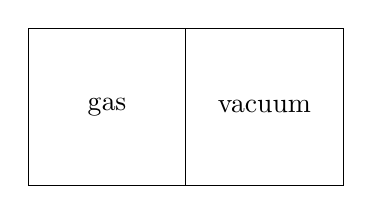
\begin{tikzpicture}
      \draw (0, 0) rectangle (4, 2);
      \draw (2, 0) -- (2, 2);
      \node at (1, 1) {gas};
      \node at (3, 1) {vacuum};
    \end{tikzpicture}
  \end{center}
  We have a valve in the partition, and as soon as we open up the valve, the gas flows to the other side of the box.

  In this system, no energy has been supplied. So $\d E = 0$. However, $\d V > 0$, as volume clearly increased. But there is no work done on or by the gas. So in this case, $-p \;\d V$ is certainly not the work done. Using the first law, we know that
  \[
    T \;\d S = p \;\d V.
  \]
  So as the volume increases, the entropy increases as well.
\end{eg}

We now revisit the concept of heat capacity. We previously defined it as $\d E/\d T$, but now we need to decide what we want to keep fixed. We can keep $V$ fixed, and get
\[
  C_V = \left(\frac{\partial E}{\partial T}\right)_V = T \left(\frac{\partial S}{\partial T}\right)_V.
\]
Usually, we do not do experiments with fixed volume. If we do a chemistry experiment in a test tube, say, then the volume is not fixed, as we may produce some gases from chemical reactions. Instead, what is fixed is the pressure. We can define
\[
  C_p = T \left(\frac{\partial S}{\partial T}\right)_p.
\]
Note that at constant pressure, we cannot write this in a simple way as $\partial E/\partial T$.

\subsection{The canonical ensemble}
So far, we have been using the microcanonical ensemble. This is a system with the energy known. This is appropriate for an isolated system, where the energy cannot change.

However, most systems are \emph{not} isolated, eg. a glass of water in the room. What \emph{is} fixed is the temperature. The \emph{canonical ensemble} describes exactly that --- we know the temperature, but not energy.

Imagine we have a system $S$, and it is interacting with a much larger system $R$. We call this $R$ a \emph{heat reservoir}. Since $R$ is assumed to be large, the energy of $S$ is negligible to $R$, and we will assume $R$ always has a fixed temperature $T$. Then in this set up, the system can exchange energy without changing $T$.

As before, we let $\bket{n}$ be a basis of microstates with energy $E_n$. Let's count how many microstates there are of the combined system $S + R$ for which $S$ is in $\bket{n}$. This is just
\[
  \Omega_R(E_{\mathrm{total}} - E_n) = \exp\left(k^{-1} S_R(E_{\mathrm{total}} - E_n)\right).
\]
By assumption, we know $E_n \ll E_{total}$. So we can expand
\[
  \Omega_R(E_{\mathrm{total}}) = \exp\left(k^{-1} S_R(E_{\mathrm{total}}) - \left(\frac{\partial S}{\partial E}\right)_V E_n\right),
\]
where we assume the volume of $R$ is fixed. But we know what $\frac{\partial S_k}{\partial E}$ is --- it is just $T^{-1}$. So we finally get
\[
  \Omega_R(E_{\mathrm{total}} - E_n) = e^{k^{-1}S_R(E_{\mathrm{total}})} e^{-\beta E_n},
\]
where we define
\begin{defi}[$\beta$]\index{$\beta$}
  \[
    \beta = \frac{1}{kT}.
  \]
\end{defi}
Now the \emph{total} number of microstates of $S + R$ is
\[
  \Omega(E_{\mathrm{total}}) = \sum_n \Omega_R(E_{\mathrm{total} - E_n}) = e^{k^{-1} S_R(E_{\mathrm{total}}} \sum_n e^{-\beta E_n}.
\]
Note that we are summing over all states, not energy.

We now use the fundamental assumption of statistical mechanics that all states of $S + R$ are equally likely. Then we know the probability that $S$ is in state $\bket{n}$ is
\[
  p(n) =\frac{\Omega_R(E_{\mathrm{total}} - E_n)}{\omega(E_{\mathrm{total}})} = \frac{e^{-\beta E_n}}{\sum_k e^{-\beta E_k}}.
\]
This is called the \term{Boltzmann distribution} for the canonical ensemble. Note that in this derivation, all the details have dropped out apart form the temperature. This describes the energy distribution of a system with fixed temperature.

Note that if $E_n \gg kT = \frac{1}{\beta}$, then the exponential is small. So only states with $E_n \sim kT$ have significant probability.

Also, as $T \to 0$, we have $\beta \to \infty$, and so only the ground state can be occupied.

We now define an important quantity.
\begin{defi}[Partition function]\index{partition function}
  The \emph{partition function} is
  \[
    Z = \sum_n e^{-\beta E_n}.
  \]
\end{defi}
So we have
\[
  p(n) = \frac{e^{-\beta E_n}}{Z}.
\]
\begin{prop}
  For two non-interacting systems, we have $Z(\beta) = Z_1(\beta) Z_2(\beta)$.
\end{prop}

\begin{proof}
  Since the systems are not interacting, we have
  \[
    Z = \sum_{n, m} e^{-\beta (E_n^{(1)} + E_n^{(2)})} = \left(\sum_n e^{-\beta E_n^{(1)}}\right)\left(\sum_n e^{-\beta E_n^{(2)}}\right) = Z_1 Z_2.
  \]
\end{proof}

Note that in general, energy is \emph{not} fixed, but we can compute the average value:
\[
  \bra E\ket = \sum_n p(n) E_n = \sum \frac{E_n e^{-\beta E_n}}{Z} = -\frac{\partial}{\partial \beta} \log Z.
\]
Here we are taking the partial derivative with all $E_i$ fixed. Usually, these $\{E_i\}$ depend on just a few ``external parameters'', such as the volume $V$, magnetic field $B$, \ldots. It also depends on other microscopic things such as masses of atoms, but we cannot control those.

We look at the simple case where $V$ is the only parameter we can vary. Then $Z = Z(\beta, V)$. Then we can rewrite
\[
  \bra E \ket = - \left(\frac{\partial}{\partial \beta} \log Z\right)_V.
\]
This gives us the average, but we also want to know the variance of $E$. We have
\[
  \Delta E^2 = \bra (E - \bra E\ket)^2 \ket = \bra E^2\ket - \bar E\ket^2.
\]
On the first example sheet, we calculate that this is in fact
\[
  \Delta E^2 = \left(\frac{\partial^2}{\partial \beta^2} \log Z\right)_V = - \left(\frac{\partial \bra E\ket}{\partial \beta}\right)_V.
\]
We can now convert $\beta$-derivatives to $T$-derivatives using the chain rule. We have
\[
  \Delta E^2 = kT^2 \left(\frac{\partial \bra E\ket}{\partial T}\right)_V = kT^2 C_V.
\]
So the fluctuation around the expectation is actually proportional to the heat capacity.

From this, we can learn something important. We would expect $\bra E\ket \sim N$, the number of particles of the system. But we also know $C_V \sim N$. So
\[
  \frac{\Delta E}{\bra E\ket} \sim \frac{1}{\sqrt{N}}.
\]
Therefore, the fluctuations are negligible if $N$ is large enough. This is called the \term{thermodynamic limit} $N \to \infty$. In this limit, we can ignore the fluctuations in energy. So we expect the microcanonical ensemble and the canonical ensemble to give the same result. And for all practical purposes, $N \sim 10^{23}$ is a large number.

Because of that, we are often going to just write $E$ instead of $\bra E\ket$.

\begin{eg}
  Suppose we had particles with
  \[
    E_{\uparrow} = \varepsilon,\quad E_{\downarrow} = 0.
  \]
  So for one particle, we have
  \[
    Z_1 = \sum_n e^{-\beta E_n} = 1 + e^{-\beta \varepsilon} = 2 e^{-\beta \varepsilon/2} \cosh \frac{\beta \varepsilon}{2}.
  \]
  If we have $N$ non-interacting systems, then since the partition function is multiplicative, we have
  \[
    Z = Z_1^N = 2^n e^{-\beta \varepsilon N/2} \cosh^N \frac{\beta \varepsilon}{2}.
  \]
  From the partition function, we can compute
  \[
    \bra E \ket = - \frac{\d \log Z}{\d \beta} = \frac{N\varepsilon}{2}\left(1 - \tanh \frac{\beta \varepsilon}{2}\right).
  \]
  We can see that this agrees with the value we computed with the microcanonical ensemble, but the calculation is much easier.
\end{eg}

How do we calculate entropy for a canonical ensemble? More generally, how do we define entropy for a general probability distribution $p(n)$? There is a neat trick we can use to answer this question, which uses the meaning of the word ``ensemble''.

Recall that we have $W \gg 1$ copies of the world with $Wp(n)$ copies in the state $\bket{n}$. We apply the Boltzmann definition
\[
  S = k \log \Omega
\]
to the whole ensemble, where $\Omega$ is the number of ways of choosing which copy is in which state. This is just
\[
  \Omega = \frac{W!}{\prod_n (W p(n))!}.
\]
Using the Boltzmann definition of entropy, we can use Stirling's approximation, and find that
\[
  S_{\mathrm{ensemble}} = -kW \sum_n p(n) \log p(n).
\]
This suggests that we should define the entropy of a single copy as follows
\[
  S = -k \sum_n p(n) \log p(n).
\]
This is the \term{Gibbs entropy} of an arbitrary probability distribution.

If the density operator is given by
\[
  \hat{\rho} = \sum_n p(n) \bket{n}\brak{n},
\]
then we have
\[
  S = - \Tr(\hat{\rho} \log \hat{\rho}).
\]
We now check that this definition makes sense, in that when we have a microcanonical ensemble, we do get what we expect.
\begin{eg}
  In the microcanonical ensemble, we have
  \[
    p(n) =
    \begin{cases}
      \frac{1}{\Omega(E)} & E \leq E_n \leq E + \delta E\\
      0 & \text{otherwise}
    \end{cases}
  \]
  Then we have
  \[
    S = -k \sum_{n: E \leq E_n \leq E + \delta E} \frac{1}{\Omega(E)} \log \frac{1}{\Omega(E)} = -k \Omega(E)  \frac{1}{\Omega(E)} \log \frac{1}{\Omega(E)} = k \log \Omega(E).
  \]
  So the Gibbs entropy reduces to the Boltzmann entropy.
\end{eg}

How about the canonical ensemble?
\begin{eg}
  In the canonical ensemble, we have
  \[
    p(n) = \frac{e^{-\beta E_n}}{Z}.
  \]
  Plugging this into the definition, we find that
  \begin{align*}
    S &= -k \sum_n p(n) \log \left(\frac{e^{-\beta E_n}}{Z}\right)\\
    &= -k \sum_n p(n) (-\beta E_n - \log Z)\\
    &= k \beta \bra E\ket = k\log 2,
  \end{align*}
  using the fact that $\sum p(n) = 1$.

  Using the formula of the expected energy, we find that this is in fact
  \[
    S = k \frac{\partial}{\partial T} (T \log Z)_V.
  \]
\end{eg}
\subsection{Maximizing entropy}
We can ask ourselves --- what probability distribution maximizes the entropy? It turns out we end up getting the different ensembles we've got as we put different constraints.

If we maximize $S_{\mathrm{Gibbs}}$ over all probability distributions such that $p(n) = 0$ unless $E \leq E_n \leq E + \delta E$. Of course, we also have the constraint $\sum p(n) = 1$. So we can use a Lagrange multiplier $\alpha$ and extremize
\[
  k^{-1}S_{\mathrm{Gibbs}} + \alpha \left(\sum_n p(n) - 1\right),
\]
Differentiating with respect to $p(n)$ and solving, we get
\[
  p(n) = e^{\alpha - 1}.
\]
In particular, this is independent of $n$. So all microstates with energy in this range are equally likely, and this gives the microcanonical ensemble.

What about the canonical ensemble? To obtain this, we maximize the entropy over all $p(n)$ such that $\bra E\ket$ is fixed. The computation is on the first example sheet.

In the microcanonical ensemble, we discussed the second law of thermodynamics, namely the entropy increases with time and the maximum is achieved in an equilibrium.

But this is no longer true in the case of the canonical ensemble, because we now want to maximize the total entropy of the system plus the heat bath, instead of just the system itself. Then is there a proper analogous quantity for the canonical ensemble?

The answer is given by the \emph{free energy}. In the canonical ensemble, the probability of energy being between $E$ and $E + \delta E$ (for $\delta E \ll kT$) is given by
\[
  p(E) = \Omega_S(E) \frac{e^{-\beta E}}{2} = \frac{1}{2} e^{k^{-1} S - \beta E}
\]
where $\Omega_S(E)$ is the number of states with energy between $E$ and $\delta E$. Here we assumed that $\delta E$ is small so that the probabilities of the different particles are similar.

We define
\[
  F = E - TS,
\]
the \term{Helmholtz free energy}. Then we have
\[
  p(E) = \frac{1}{Z} e^{-\beta F}.
\]
So in the canonical ensemble, the most likely $E$ is the one that minimizes $F$.

In general, in an isolated system, $S$ increases, and $S$ is maximized in equilibrium. In a system with a reservoir, $F$ decreases, and $F$ minimizes in equilibrium. In some sense $F$ captures the competition between entropy and energy. We will discuss this further later.

Now is there anything analogous to the first law
\[
  \d E = T \d S - p \d V?
\]
Since we have $S$ and $V$ on the right, here we are regarding energy as a function of entropy and volume, or entropy as a function of $E$ and $V$. Using this, we can write
\[
  \d F = \d E - \d(TS)  = -s \d T - p \d V.
\]
So it is natural to think of $F$ as a function of $T$ and $V$. Mathematically, the relation between $F$ and $E$ is that $F$ is the \term{Legendre transform} of $E$.

From this expression, we can immediately write down
\[
  S = - \left(\frac{\partial F}{\partial T}\right)_V,
\]
and the pressure is
\[
  p = -\left(\frac{\partial F}{\partial V}\right)_T.
\]
The final claim about the free energy is that we have a very useful formula for it. We have
\[
  F = -kT \log Z.
\]
Alternatively, 
\[
  Z = e^{-\beta F}.
\]
Let's prove this. We use the fact that
\[
  \frac{\d}{\d \beta} = kT^2 \frac{\d}{\d T}.
\]
Then we can start from
\begin{align*}
  F &= E - TS \\
  &= - \left(\frac{\partial \log Z}{\partial \beta}\right) - TS \\
  &= kT^2 \left(\frac{\partial \log Z}{\partial T}\right)_V - kT \frac{\partial}{\partial T}(T \log Z)_V\\
  &= -k T \log Z,
\end{align*}
and we are done. Good.

\subsection{The chemical potential}
So far we have considered situations where we had fixed energy or fixed volume. However, there are often other things that are fixed. For example, the number of particles, or the electric charge of the system would be fixed. If we measure these things, then this restricts which microstates are accessible.

Let's consider $N$. This quantity was held fixed in the microcanonical and canonical ensembles. But these quantities do depend on $N$, and we can write
\[
  S(E, V, N) = k \log \Omega(E, V, N).
\]
Previously, we took this expression, and asked what happens when we varied $E$, and we got temperature. We then asked what happens when we vary $V$, and we got pressure. Now we ask what happens when we vary $N$.
\begin{defi}[Chemical potential]\index{chemical potential}
  The \emph{chemical potential} of a system is given by
  \[
    \mu = -T \left(\frac{\partial S}{\partial N}\right)_{E, V}.
  \]
\end{defi}

Why is this significant? Recall that when we only varied $E$, then we figured that two systems in equilibrium must have equal temperature. Then we varied $V$ as well, and found that two systems in equilibrium must have equal temperature \emph{and} pressure. Then it shouldn't be surprising that if we have two interacting systems that can exchange particles, then we must have equal temperature, pressure \emph{and} chemical potential. Indeed, the same argument works.

If we want to consider what happens to the first law when we vary $N$, we can just straightforwardly write
\[
  \d S = \left(\frac{\partial S}{\partial E}\right)_{V, N} \d E + \left(\frac{\partial S}{\partial V}\right)_{E, N} \d V + \left(\frac{\partial S}{\partial N}\right)_{E, V} \d V.
\]
Then as before, we get
\[
  \d E = T \;\d S - p \;\d V + \mu \;\d N.
\]
From this expressions, we can get some feel for what $\mu$ is. This is the energy cost of adding one particle at $S, V$. We will actually see later that $\mu$ is actually negative, as it is hard to add a particle keeping the entropy fixed.

Note that if we change $N$ to $Q$, then $\mu$ changes into $\Phi$, the electrostatic potential.

From the first law, we can write
\[
  \mu = \left(\frac{\partial E}{\partial N}\right)_{S, V}.
\]
We might ask, can we obtain this result from the original definition directly? Indeed, we can, using the magic identity
\[
  \left(\frac{\partial x}{\partial y}\right)_z \left(\frac{\partial y}{\partial z}\right)_x \left(\frac{\partial z}{\partial x}\right)_y = -1.
\]
In the canonical ensemble, we have fixed $T$, but the free energy will also depend on energy:
\[
  F(T, V, N) = E - TS.
\]
Again, we have
\[
  \d F = \d E - \d (TS) = -S\;\d T - p\;\d V + \mu\;\d N.
\]
So we have
\[
  \mu = \left(\frac{\partial F}{\partial N}\right)_{T, V}.
\]
\subsection{Grand canonical ensemble}
Consider a system $S$ in equilibrium with a ``heat and particle'' reservoir $R$, with which it can exchange both heat and particles. Again, $\mu$ and $T$ are fixed by their values in $R$. We repeat the argument with the canonical ensemble, and we will find that the probability that a system is in state $n$ is
\[
  p(n) = \frac{e^{-\beta (E_n - \mu N_n)}}{\mathcal{Z}},
\]
where $N_n$ is the number of particles in $\bket{n}$, and
\[
  \mathcal{Z} = \sum_n e^{-\beta(E_n- \mu N_n)}
\]
is the \term{grand canonical partition function}.
\printindex
\end{document}
